\documentclass{article}
\usepackage[utf8]{inputenc}

%\usepackage[top=25mm,left=25mm,right=25mm,bottom=25mm,a4paper,nohead]{geometry}


\usepackage{amsmath}
\usepackage{amsfonts}
\usepackage{amssymb}
\usepackage{dsfont}
\usepackage{color}


\usepackage{tikz}
\tikzstyle{texto}=[inner sep=0pt,minimum size=14pt]
\tikzstyle{diagramC}=[ellipse,x readius=6,y radius=8, thick]

\newtheorem{definition}{Definition}
\newtheorem{example}[definition]{Example}

\newcommand{\cred}[1]{{\color{red}#1}}

\begin{document}



\title{Marlo Diagrams: representation and operations}
\author{}
%\date{}

\maketitle

\begin{abstract}
    Some notes to fix the structure of the diagrams and behaviour of the operations prior to the implementation of a visual reasoning assistant. 
\end{abstract}

\section{Diagram structure}

\begin{definition}[Literals]
Let $P$ be a set of propositional variables. Given $p\in P$, both $p$ and $\lnot p$ are \emph{literals}. Literals $p$ and $\lnot p$ are \emph{complementary literals}. Given a literal $\lambda$ (like $p$ or $\lnot p$), $\overline{\lambda}$ denotes its complementary literal ($\lnot p$ or $p$, respectively). The set of literals built from $P$ is $Lit(P)$. A set of literals is \emph{consistent} if it does not contain complementary literals. 
\end{definition}

\begin{definition}[Diagram]
A \emph{diagram} $D=\left<S,A,I,O\right>$ has the following structure:
\begin{itemize}
    \item $S\in Lit(P)$, the ``\emph{subject}'' of $D$.
    \item $A\subset Lit(P)-\{S\}$ with $|A|\in\mathds{N}$, the ``\emph{all}'' of $D$. 
    \item $I\subset \mathcal{P}\left(Lit(P)-(A\cup\{S\})\right)$ with $|I|\in \mathds{N}-\{0\}$ and $|\cup I|\in \mathds{N}$, the ``\emph{in}'' of $D$.
    \item $O\subset A\cup (\cup I)$ with $|O|\in \mathds{N}$, the ``\emph{out}'' of $D$.
\end{itemize}
\end{definition}

\begin{definition}[Consistent Diagram]
A diagram $D=\left<S,A,I,O\right>$ is \emph{consistent} iff for all $R\in I$, the set of literals $\{S\}\cup A\cup R$ is consistent. 
\end{definition}

\begin{definition}[Scope]
Given a diagram $D=\left<S,A,I,O\right>$, the \emph{scope} of $D$, denoted as $Sc(D)$ is the set of propositions appearing in the diagram, that is,
\[Sc(D) = \{S\} \cup A \cup (\cup I).\]
\end{definition}

\subsection{Examples}

\begin{example}[All $a$ are $b$]
\label{ex1}
The diagram for ``All 
$a$ (universal) are $b$ (particular)'' is 
$D=\left<a,\{b\}, \{\varnothing\}, \{b\}\right>$.
\end{example}

\begin{example}[Some $a$ are $b$] 
\label{ex2}
The diagram for ``Some 
$a$ (particular) are $b$ (particular)'' is 
$D=\left<a,\varnothing, \{\{b\},\varnothing\}, \{b\}\right>$.
\end{example}

% Puedes copiar y pegar de este

\subsection{Definición de las conectivas por Marcos}

\cred{** Revisar, en las partes $O$ se confunde $\varnothing$ con $\{\varnothing\}$. Para hablar de equivalencia (y, sobre todo, justificarlas) es necesaria una semántica. O bien, una vez dadas las operaciones probar que se puede ir de cada variante a las demás mediante transformación y conversión.}

\begin{example}[$a$ iff b]
The diagrams for biconditional ``$a \leftrightarrow b$''  are
\[
\begin{array}{rclcl}
D &=& \left<\ a,\{ b\}, \{\varnothing\}, \varnothing\right> 
& \equiv & \left<\ b,\{a\}, \{ \varnothing\}, \varnothing\right> \\
& \equiv & \left< \lnot b,\{\lnot a \}, \{\varnothing\}, \varnothing\right> & \equiv & \left< \lnot a,\{\lnot b\}, \{ \varnothing\}, \varnothing\right>.
\end{array}\]
\end{example}

\begin{example}[$a \veebar b$] 
The diagrams for exclusive disjunction ``$a \veebar  b$'' are
\[
\begin{array}{rclcl}
D&=& \left<\ a,\{ \lnot b\}, \{\varnothing\}, \varnothing\right> & \equiv & \left<\lnot b,\{a\}, \{ \varnothing\}, \varnothing\right>\\
& \equiv & \left< \ b,\{\lnot a \}, \{\varnothing\}, \varnothing\right> & \equiv & \left< \lnot a,\{\ b\}, \{ \varnothing\}, \varnothing\right>.
\end{array}\]
\end{example}


\begin{example}[$a \to b$ (conditional)] 
The  diagram for ``$a \to  b$'' (conditional) is 
\[
\begin{array}{rclcl}
D&=&\left<\ a,\{b\}, \{\varnothing\}, \{b\}\right>& \equiv& \left<\ b,\{\varnothing\}, \{ a\}, \varnothing\right> \\ & \equiv & \left< \lnot a,\{ \lnot b \}, \{\varnothing\}, \{ \lnot b\}\right> & \equiv & \left< \lnot b ,\{ \varnothing\}, \{ a\},  \varnothing\right>.
\end{array}\]
\end{example}

\begin{example}[$a  \vee b$ (inclusive)] 
The diagram for inclusive disjunction``$a \vee b$'' are
\[
\begin{array}{rclcl}
D&=&\left<\lnot a,\{b\}, \{\varnothing\}, \{b\}\right> & \equiv& \left<\ b,\{\varnothing\}, \{ \lnot a\}, \varnothing\right>\\ & \equiv &\left< \lnot b,\{ a \}, \{\varnothing\}, \{ a\}\right> & \equiv & \left< \ a,\{ \varnothing\}, \{ \lnot b\},  \varnothing\right>.
\end{array}\]
\end{example}

\begin{example}[$a$ Nand $b$] 
The diagrams for ``$a$ Nand $b$''  are 
\[
\begin{array}{rclcl}
D & = & \left<\ a,\{\lnot b\}, \{\varnothing\}, \{\lnot b\}\right> & \equiv &  \left<\lnot b,\{\varnothing\}, \{ a\}, \varnothing\right>\\ &  \equiv & \left< \ b,\{\lnot a \}, \{\varnothing\}, \{\lnot  a\}\right> & \equiv & \left< \lnot a,\{\varnothing\}, \{ b\}, \varnothing\right>.
\end{array}\]
\end{example}


\begin{example}[$a$ or $b$ (inclusive)] 
The diagram for ``$a$ or $b$'' (inclusive disjunction) is 
$D=\left<\lnot a,\{b\}, \{\varnothing\}, \{b\}\right>$.
\end{example}


\begin{example}[or $a$ or $b$ (exclusive)] 
The diagram for ``$a$ or $b$'' (exclusive disjunction) is 
$D=\left<\lnot a,\{b\}, \{\varnothing\}, 
\varnothing \right>$.
\end{example}


\subsection{Graphical representation}

\cred{** TODO: Explain the representation of the diagrams.}

\begin{figure}[htbp!]
    \centering
    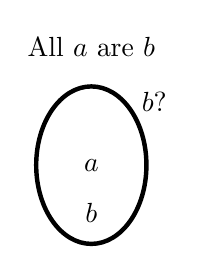
\begin{tikzpicture}[thick]
    \draw [ultra thick] (0,0.5) ellipse [x radius = 0.7cm, y radius = 1cm];
    \node [texto] (t3)  at (0,  0.5) {$a$};
    \node [texto] (t3)  at (0,  -0.1) {$b$};
    \node [texto] (t3)  at (0.8,  1.3) {$b?$};
    \node [texto] (t3)  at (0,  2) {All $a$ are $b$};
    \end{tikzpicture}\hspace{2cm}
    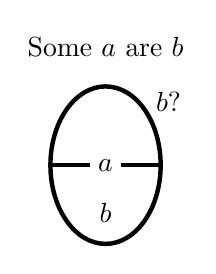
\begin{tikzpicture}[thick]
    \draw [ultra thick] (0,0.5) ellipse [x radius = 0.7cm, y radius = 1cm];
    \draw [ultra thick] (-0.7,0.5) -- (-0.2,0.5);
    \draw [ultra thick] (.7,0.5) -- (0.2,0.5);
    \node [texto] (t3)  at (0,  0.5) {$a$};
    \node [texto] (t3)  at (0,  -0.1) {$b$};
    \node [texto] (t3)  at (0.8,  1.3) {$b?$};
    \node [texto] (t3)  at (0,  2) {Some $a$ are $b$};
    \end{tikzpicture}
    \caption{Diagrams for examples~\ref{ex1} and~\ref{ex2}.}
    \label{fig:initExamples}
\end{figure}

Figure~\ref{fig:initExamples} shows the graphical representation of the diagrams in examples~\ref{ex1} and~\ref{ex2}. 

\subsection{Translation into FOL}

\cred{** TODO: Explain the general idea of the translation.}

\cred{Idea: Existence for $x\cup S$ when $x\in I$ and $x\cap O \neq\varnothing$.}

The translation of the diagram in example~\ref{ex1} into FOL is:
\[
\forall x (Ax \to Bx) \,\cred{\land\, \exists x Ax} 
\]

The translation of the diagram in example~\ref{ex2} into FOL is:
\[
\exists x (Ax \land Bx)
\]

The translation of the diagram
$D=\left<a,\varnothing, \{\{b\},\varnothing\}, \varnothing\right>$ (like the one in the right of Fig.\ref{fig:initExamples} but without $b?$ in the outer part) is
\[
\exists x (Ax \land Bx) \land \forall x (Bx \to Ax)
\]

The translation of the  diagram 
$D=\left<a,\{b\}, \{\varnothing, \{c\}\},\{b\}\right>$ is
\[
\forall x (Ax \to Bx) \land \exists x (Ax \land Cx) \land \forall x (Cx\to Ax)
\]
And the representation:
\begin{center}
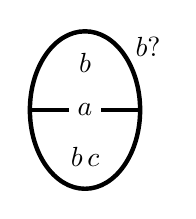
\begin{tikzpicture}[thick]
    \draw [ultra thick] (0,0.5) ellipse [x radius = 0.7cm, y radius = 1cm];
    \draw [ultra thick] (-0.7,0.5) -- (-0.2,0.5);
    \draw [ultra thick] (.7,0.5) -- (0.2,0.5);
    \node [texto] at (0,  0.5) {$a$};
    \node [texto] at (0,  -0.1) {$b\,c$};
    \node [texto] at (0,  1.1) {$b$};
    \node [texto] at (0.8,  1.3) {$b?$};
\end{tikzpicture}
\end{center}


\section{Operations on Marlo Diagrams}

\subsection{Conversion}

\cred{*** Esto hay que revisarlo con cuidado y poner muchos ejemplos.}

\begin{definition}[Conversion]
Given $D=\left< S, A, I, O\right>$, the conversion of $D$ for $S'$ produces 
$Conv(D,S')=\left<S', A', I', O'\right>$ iff
\begin{eqnarray*}
S' & \in & A \cup (\cup I)\\
A' & = & \left\{ 
\begin{array}{ll}
    \varnothing &  if \quad S'\in O\\
    \{S\}\cup (A -\{S'\})\cup &\\
    ((\cup I-\{S'\})\cap (\cap \{x -\{S'\}\mid x\in I\, \& \, S'\in x\}))& otherwise
\end{array}
\right.\\
I' &=& \left\{
\begin{array}{ll}
    \{((x-\{S'\})\cup \{S\}\cup A)- A' \mid x\in I\} & if\quad S'\in A \\
    \{((x-\{S'\})\cup \{S\} \cup A)- A' \mid x\in I\, \& \, S'\in x \} & otherwise
\end{array}
\right.\\
& \cup & \left\{
\begin{array}{ll}
    \{\varnothing\} & if\quad S'\in O \\
    \varnothing &  otherwise
\end{array}
\right.\\
O' &=& \left((O-\{S'\}) \cup (\cup \{x\cup A \cup \{S\} \mid x\in I \, \& \, S'\notin (x\cup A)\})\right)\\
& \cap & (A' \cup (\cup I'))
\end{eqnarray*}
\end{definition}

\subsection{Transformation}

\begin{definition}[Transformation]
Given a diagram $D$, the \emph{transformation} of $D$ produces $Tr(D)$ in two cases:
\begin{itemize}
    \item $D = \left< \gamma, \{\lambda\}, \{\varnothing\}, O\right>$. Then,
    \[
    Tr(D) = 
    \left<
    \overline{\lambda}, \{\overline{\gamma}\},
    \{\varnothing\}, O'
    \right>,
    \]
    with 
    \[
    O' = \left\{
    \begin{array}{ll}
        \varnothing & \text{if}\quad O = \varnothing \\
        \{\overline{\gamma}\} & \text{otherwise (that is, $O=\{\lambda\}$)} 
    \end{array}\right.
    \]
    \item $D = \left< \gamma, \varnothing, \{\{\lambda\},\varnothing\}, \varnothing\right>$. Then,
    \[
    Tr(D) = 
    \left<
    \overline{\lambda}, \varnothing,
    \{\{\overline{\gamma}\},\varnothing\}, \varnothing\right>.
    \]
\end{itemize}
\end{definition}

\subsection{Inference}

\begin{definition}[Inference]
Given the diagrams
\[D_1 = \left< s, A_1, I_1, O_1\right>\quad\quad
\text{and}\quad\quad
D_2 = \left< s, A_2, I_2, O_2\right>,
\]
the inference with $D_1$ and $D_2$ produces
\[D_3 = D_1 \oplus D_2 = \left< s, A_1 \cup A_2, I_3, O_3
\right>,\]
with 
\begin{eqnarray*}
I_3 & = & 
\{x-A_2 \mid x\in I_1\} \cup
\{x-A_1 \mid x\in I_2\} \\
O_3 & = &  
\left(O_1 - \left(Sc\left(D_2\right)-O_2\right) \right) \cup
\left(O_2 - \left(Sc\left(D_1\right)-O_1\right) \right).
\end{eqnarray*}


\end{definition}

\begin{example}
\label{exInf}
Consider the following diagrams: 
\begin{eqnarray*}
D_1 & = & \left<a, \{b\}, \{\{c\},\varnothing\}, \{b,c\}    \right>\\
D_2 & = & \left<a, \varnothing, \{\{b,d\},\varnothing\}, \{d\}    \right>.
\end{eqnarray*}
The inference with $D_1$ and $D_2$ (view Figure~\ref{fig:InfEx}) produces
\begin{eqnarray*}
D_1\oplus D_2 & = & \left<a, \{b\}, \{\{c\},\{d\},\varnothing\}, \{c,d\}\right>.
\end{eqnarray*}
\end{example}

\begin{figure}
    \centering
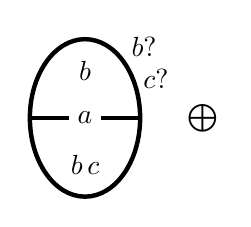
\begin{tikzpicture}[thick]
    \draw [ultra thick] (0,0.5) ellipse [x radius = 0.7cm, y radius = 1cm];
    \draw [ultra thick] (-0.7,0.5) -- (-0.2,0.5);
    \draw [ultra thick] (.7,0.5) -- (0.2,0.5);
    \node [texto] at (0,  0.5) {$a$};
    \node [texto] at (0,  -0.1) {$b\,c$};
    \node [texto] at (0,  1.1) {$b$};
    \node [texto] at (0.75,  1.4) {$b?$};
    \node [texto] at (0.9,  1) {$c?$};
    \node [texto] at (1.5,  0.5) {$\bigoplus$};
\end{tikzpicture}\quad\,
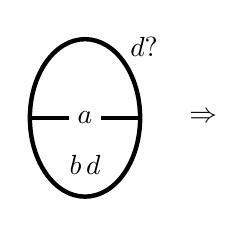
\begin{tikzpicture}[thick]
    \draw [ultra thick] (0,0.5) ellipse [x radius = 0.7cm, y radius = 1cm];
    \draw [ultra thick] (-0.7,0.5) -- (-0.2,0.5);
    \draw [ultra thick] (.7,0.5) -- (0.2,0.5);
    \node [texto] at (0,  0.5) {$a$};
    \node [texto] at (0,  -0.1) {$b\,d$};
    \node [texto] at (0.75,  1.4) {$d?$};
    \node [texto] at (1.5,  0.5) {$\Rightarrow$};
\end{tikzpicture}
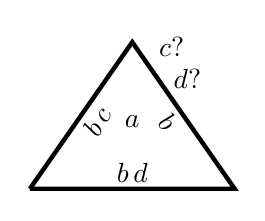
\begin{tikzpicture}[thick]
    \draw [ultra thick] (-1.3,-1.3) -- (1.3,-1.3) -- (0,0.562) -- (-1.3,-1.3);
    \node [texto] at (0,  -0.45) {$a$};
    \node [texto] at (0,  -1.1) {$b\,d$};
    \node [rotate=60,texto] at (-0.45,  -.45) {$b\,c$};
    \node [texto,rotate=-45] at (0.45,  -.45) {$b$};
    \node [texto] at (0.5,  .5) {$c?$};
    \node [texto] at (0.7,  .1) {$d?$};
\end{tikzpicture}
    \caption{Example of inference (example~\ref{exInf}).}
    \label{fig:InfEx}
\end{figure}

\subsection{Extraction}

\begin{definition}[Extraction]
Given the diagram $D=\left< S,A,I,O\right>$ and $\lambda \in A \cup (\cup I)$, the \emph{extraction of $\lambda$ in $D$} produces
\[
Elim(D,\lambda) = \left< S, A- \{\lambda\}, \{x-\{\lambda\}\mid x \in I \}, O- \{\lambda\}\right>.
\]
\end{definition}

\end{document}

%%% Local Variables:
%%% mode: latex
%%% TeX-master: t
%%% End:
